\documentclass[aspectratio=169, table]{beamer}

%\usepackage[beamertheme=./praditatheme]{Pradita}
\usepackage[utf8]{inputenc}

\usetheme{Pradita}

\subtitle{MTI102-Information System \&\\Technology Architecture}
\title{\vskip-0.7cm \Large Phase F: Migration Plan\\in TOGAF
	Architecture\\Development Method (ADM)}
\date[Serial]{\scriptsize {PRU/SPMI/FR-BM-18/0222}}
\author[Pradita]{\small {\textbf{Alfa Yohannis}}}

\begin{document}
	
	\frame{\titlepage}
	
	\begin{frame}
		\frametitle{Aims}
		\begin{enumerate}
			\item Finalize the Architecture Roadmap and the supporting Implementation and Migration Plan
			\item Ensure that the Implementation and Migration Plan is coordinated with the enterprise’s approach to managing and implementing change in the enterprise’s overall change portfolio
			\item Ensure that the business value and cost of work packages and Transition Architectures are understood by key stakeholders
		\end{enumerate}		
	\end{frame}
	
	\begin{frame}
		\frametitle{Inputs}
		\vspace{22pt}
		\begin{columns}[onlytextwidth]
			\begin{column}{0.45\textwidth}
				\begin{enumerate}
					\item Request for Architecture Work
					\item Communications Plan
					\item Organizational Model for Enterprise Architecture
					\item Governance Models and Frameworks
					\item Tailored Architecture Framework
					\item Statement of Architecture Work
					\item Architecture Vision
					\item Architecture Repository
					\item Draft Architecture Requirements Specification
				\end{enumerate}
				
			\end{column}
			\begin{column}{0.55\textwidth}
				\begin{enumerate}
					\setcounter{enumi}{8}
					\item Draft Architecture Definition Document, including:
					\begin{enumerate}
						\item Transition Architectures, if any
					\end{enumerate}
					\item Change Requests for existing programs and projects
					\item Architecture Roadmap, including:
					\begin{enumerate}
						\item Identification of work packages
						\item Identification of Transition Architectures
						\item Implementation Factor Assessment and Deduction Matrix
					\end{enumerate}
					\item Capability Assessment
					\item Implementation and Migration Plan (outline)
				\end{enumerate}
			\end{column}
		\end{columns}
	\end{frame}
	
	
	\begin{frame}
		\frametitle{Steps}
		\vspace{20pt}
		\begin{enumerate}
			\item Confirm management framework interactions for the Implementation and Migration Plan
			\item Assign a business value to each work package
			\item Estimate resource requirements, project timings, and availability/delivery vehicle
			\item Prioritize the migration projects through the conduct of a cost/benefit assessment and risk validation
			\item Confirm Architecture Roadmap and update Architecture Definition Document
			\item Complete the Implementation and Migration Plan
			\item Complete the architecture development cycle and document lessons learned
		\end{enumerate}
	\end{frame}
	
	\begin{frame}
		\frametitle{Step 1: Confirm Management Framework Interactions}
		\framesubtitle{for the Implementation and Migration Plan}
		\vspace{20pt}
			\begin{enumerate}
				\item Coordinate the Implementation and Migration Plan with the organization's management frameworks.
				\item The plan should impact four management frameworks: Business Planning, Enterprise Architecture, Portfolio/Project Management, and Operations Management.
				\item Understand and integrate the plan into each framework's plans.
				\item The Implementation and Migration Plan might become part of another plan, possibly produced by the Enterprise Architecture framework.
			\end{enumerate}
	\end{frame}

	\begin{frame}
		\frametitle{Step 2: Assign a Business Value to Each Work Package}
		\framesubtitle{\hspace{1cm}}
		\vspace{20pt}
			\begin{enumerate}
				\item Establish and assign business values to work packages and projects.
				\item Utilize Capability-Based Planning if applicable for assigning business values.
				\item Address Performance Evaluation Criteria and Return-on-Investment Criteria for monitoring progress and resource allocation.
				\item Define Critical Success Factors and Measures of Effectiveness for project success.
				\item Consider Strategic Fit with the enterprise architecture when approving projects and determining deliverable value.
			\end{enumerate}
	\end{frame}

	\begin{frame}
	\frametitle{Step 3: Estimate resource requirements, project timings, and}
	\framesubtitle{availability/delivery vehicle}
	\vspace{20pt}
		\begin{enumerate}
			\item Determine required resources, timelines, and cost estimates for each project and their increments.
			\item Break down costs into capital and operations/maintenance categories.
			\item Identify opportunities to offset costs through decommissioning existing systems.
			\item Assign necessary resources to each activity and aggregate them at project increment and project levels.
		\end{enumerate}
\end{frame}

	\begin{frame}
	\frametitle{Step 4: Prioritize the migration projects through}
	\framesubtitle{the conduct of a cost/benefit assessment and risk validation}
	\vspace{20pt}
		\begin{enumerate}
			\item Prioritize projects based on their business value and delivery cost, considering net benefits and risk mitigation.
			\item Ensure all costs are accounted for and decision-makers understand the long-term net benefits.
			\item Review and update the project list with risk-related comments.
			\item Obtain stakeholder agreement on project prioritization using criteria from the draft Architecture Roadmap and individual agendas.
			\item Formally review and revise the risk assessment, ensuring a clear understanding of residual risk and projected funding.
		\end{enumerate}
\end{frame}

	\begin{frame}
	\frametitle{Step 5: Confirm Architecture Roadmap and}
	\framesubtitle{update Architecture Definition Document}
	\vspace{20pt}
		\begin{enumerate}
			\item Update the Architecture Roadmap with Transition Architectures.
			\item Assess time-spans between Transition Architectures based on business value, capability increments, and risk factors.
			\item Consolidate deliverables for each Transition Architecture by project increment, resulting in a revised Architecture Roadmap.
			\item Update the Architecture Definition Document, aligning projects and objectives with Transition Architectures, and creating an Architecture Definition Increments Table if needed.
		\end{enumerate}
\end{frame}

\begin{frame}
	\frametitle{Step 5-1: Architecture Definition Increments Table}
	\framesubtitle{\hspace{1cm}}
\vspace{25pt}
\begin{columns}[onlytextwidth]
	\begin{column}{0.45\textwidth}
		\begin{enumerate}
			\item \textbf{Confirm Architecture Roadmap and update Architecture Definition Document}
			\begin{enumerate}
				\setcounter{enumi}{4}
				\item Create an Architecture Definition Increments Table to plan Transition Architectures and track the enterprise architecture's status at specified times.
				\item Draw up a table listing projects and their incremental deliverables across the Transition Architectures.
			\end{enumerate}
		\end{enumerate}
	\end{column}
	\begin{column}{0.55\textwidth}
		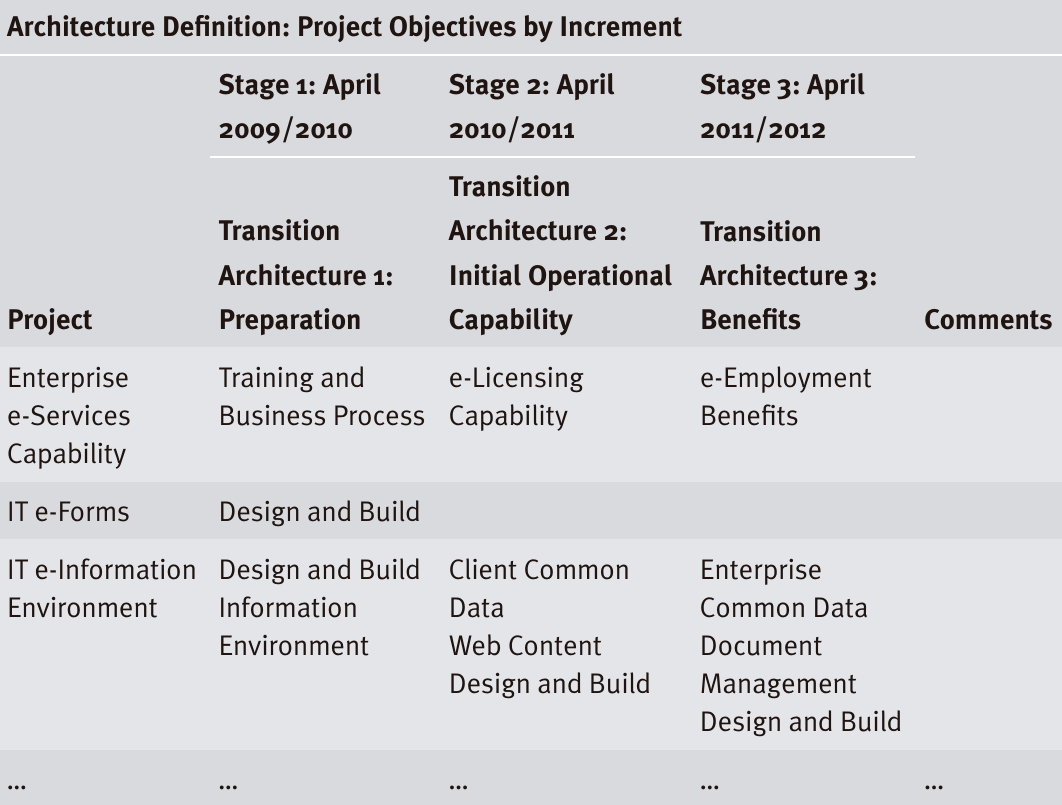
\includegraphics[width=\textwidth]{../figures/architecture_definition_increments.png}
	\end{column}
\end{columns}

\end{frame}

			

	\begin{frame}
		\frametitle{Step 6: Complete the Implementation and Migration Plan}
		\framesubtitle{\hspace{1cm}}
	\vspace{20pt}
		\begin{enumerate}
			\item Generate the completed Implementation and Migration Plan, integrating gathered details using planning and management techniques.
			\item Include all projects, project increments, and activities along with their dependencies in a comprehensive project plan.
			\item Capture and assess external dependencies and overall resource availability.
			\item Use the Transition Architecture State Evolution Table to illustrate proposed states of architectures with the Technical Reference Model (TRM).
			\item Describe Solution Building Blocks (SBBs) with their delivery and impact on services, marking their progression in the enterprise architecture.
		\end{enumerate}
\end{frame}

	\begin{frame}
	\frametitle{Step 7: Complete the architecture development cycle and }
	\framesubtitle{document lessons learned}
	\vspace{20pt}
		\begin{enumerate}
			\item Transition governance from architecture development to architecture realization.
			\item Consider producing an Implementation Governance Model if the Architecture Capability is mature enough.
			\item Document lessons learned and incorporate them into the governance process in Phase H for managing the Architecture Capability.
			\item Express the detail of the Architecture Roadmap and Implementation and Migration Plan at a similar level as the Architecture Definition Document from Phases B, C, and D.
			\item If needed, iterate another ADM cycle at a lower level of detail based on the level of the Target Architecture and Implementation and Migration Plan.
		\end{enumerate}
\end{frame}


	\begin{frame}
		\frametitle{Outputs}
		\vspace{20pt}
		\begin{enumerate}
			\item Implementation and Migration Plan (detailed)
			\item Finalized Architecture Definition Document, including:
			\begin{enumerate}
				\item Finalized Transition Architectures, if any
			\end{enumerate}
			\item Finalized Architecture Requirements Specification
			\item Finalized Architecture Roadmap
			\item Re-Usable Architecture Building Blocks (ABBs)
			\item Requests for Architecture Work for a new iteration of the ADM cycle (if any)
			\item Implementation Governance Model
			\item Change Requests for the Architecture Capability arising from lessons learned
		\end{enumerate}
	\end{frame}
	
	
	\begin{frame}
		\frametitle{Summary}
		\begin{enumerate}
			\item Phase F addresses migration planning, which focuses on moving from the Baseline to the Target Architectures.
			\item It includes creating the finalized Architecture Definition Document, Architecture Roadmap, and the detailed Implementation and Migration Plan.
			\item After completion of this phase, the preparation for implementation has been completed.
		\end{enumerate}
	\end{frame}
		
\end{document}
